\documentclass[a4paper, 12pt]{article}
\usepackage{graphicx,hyperref,float,comment,listings,amsmath}
\lstdefinestyle{mystyle}{
	basicstyle=\small,
	breaklines=true,
	numbers=left,
	numberstyle=\tiny,
	numbersep=5pt,
}
\lstset{style=mystyle}
\graphicspath{{images/}}
\hypersetup{
	colorlinks=true,
	linkcolor=blue,
	filecolor=magenta,      
	urlcolor=cyan,
}

\title{\Large\textbf{Supression d'imprimante et traitement des données sur le Lambda 9}}
\author{Gaëtan PINOT}
\date{Avril 2024}

\begin{document}
\pagenumbering{gobble}
%Page de titre
\maketitle

\newpage

\pagenumbering{arabic}

\section{Cablage}\label{cablage}

La station de traitement de données du Lambda 9 est normalement connéctée à une imprimante part un port DB25, le standard de communication entre les deux est RS232.
Le standard RS232 permet d'utiliser un port série standard DE9\footnote{DE9 est le nom correct du port plus souvent appelé DB9 %\url{https://fr.wikipedia.org/wiki/D-sub}
}.
Pour pouvoir remplacer l'imprimante par un ordinateur il faut un cable de conversion entre le port DB25 et le port DB9 de l'ordinateur.


\begin{table}[htb]
	\begin{tabular}{|c|c|}
		\hline
		Signal & N° de pin DB25 \\ \hline
		TD     & 2              \\ \hline
		RD     & 3              \\ \hline
		RTS    & 4              \\ \hline
		CTS    & 5              \\ \hline
		DSR    & 6              \\ \hline
		GND    & 1,7            \\ \hline
		CD     & 8              \\ \hline
		RESET  & 15             \\ \hline
		DTR    & 20             \\ \hline
	\end{tabular}
	\centering
	\caption{Schéma de cablage de la sortie imprimante du Lambda 9, directement tiré des dessins techniques}
	\label{table:pinoutLambda}
\end{table}

Les deux appareils sont des DTE\footnote{Data Terminal Equipement}, les convertisseurs classiques ne fonctionnent donc pas, car certains cables doivent être croisés et certains signaux ne peuvent pas être généré par aucun des deux appareils.
Il faut un cable null-modem\footnote{Cable qui croisent certains signaux permettant la communication entre DTE} DE9-DB25.


%%%
\begin{comment}
	\begin{figure}[htb]
		\centering
		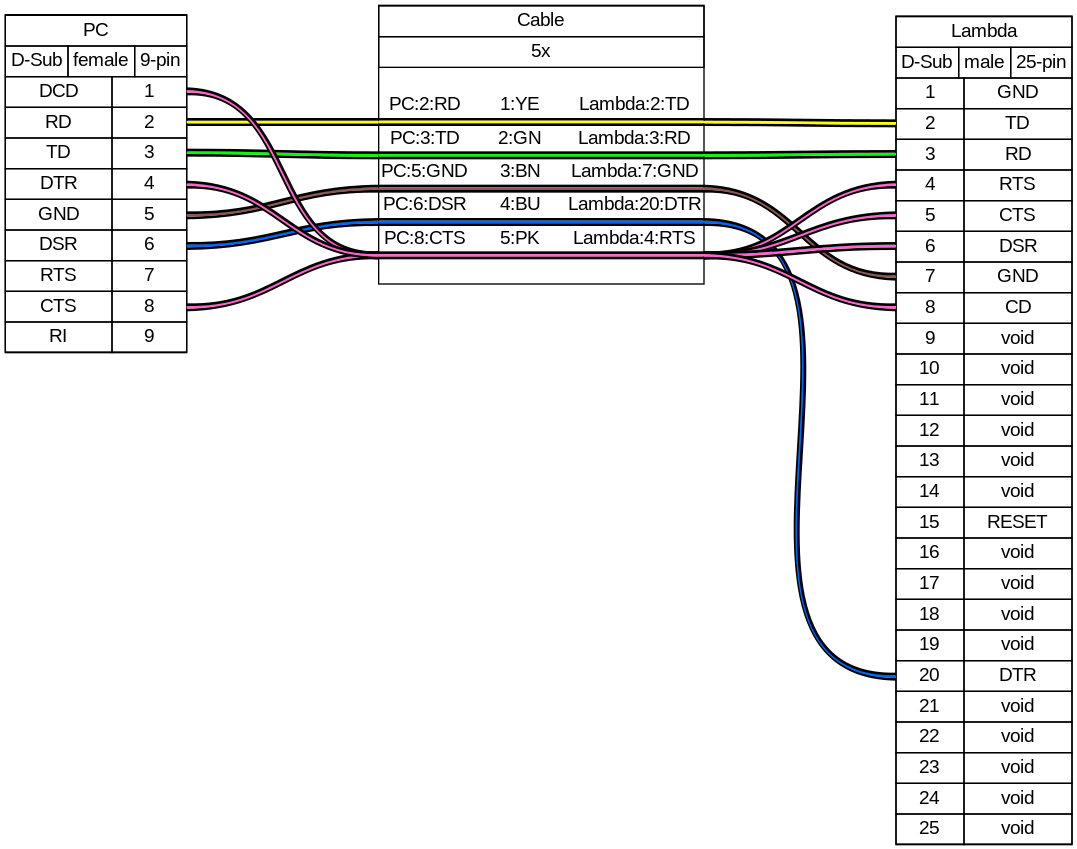
\includegraphics[width=1\textwidth]{cableLambda.png}
		\caption{Schéma de cablage entre l'ordinateur et le Lambda 9 \protect \footnotemark}
		\label{fig:cableLambda}
	\end{figure}
	\footnotetext{Schéma généré grâce à WireViz : \url{https://github.com/wireviz/WireViz}}

	\begin{table}[htb]
		\centering
		\begin{tabular}{|c|c|c|c|}
			\hline
			Signaux &DB9   & DB25    & Signaux\\ \hline\hline
			RD&2     & 2       &TD\\ \hline
			TD&3     & 3       &RD\\ \hline
			GND&5     & 7       &GND\\ \hline
			DSR&6     & 20      &DTR\\ \hline
			CD,DTR,CTS&1,4,8 & 4,5,6,8 &RTS,CTS,DSR,CD\\ \hline
		\end{tabular}
	\end{table}
	Ceci (figure \ref{fig:cableLambda}) est le schéma du seul cablage que j'ai réussi à faire fonctionner.
	Les signaux \verb|TD| et \verb|RD| sont croisés pour que les deux appareils puissent communiquer.
	Les signaux \verb|CD| sur les deux appareils sont reliés à d'autre signaux car il devrait normalement être généré par le DCE (i.e.\ l'imprimante).
	Les autrs signaux (\verb|RTS|, \verb|CTS|, \verb|DSR|, \verb|DTR|) sont reliés entre eux pour que les deux appareils soit prêt dès le branchement du cable, pour simplifier le programme de récéption des données. 
\end{comment}
%%%

\newpage
\section{Programme de réception des données}\label{programme}
\subsection{Simuler l'imprimante}\label{simuler}

On commence par connecter l'ordinateur au Lambda 9 avec le cable null-modem.
Puis on met en place une connexion série entre l'ordinateur et le Lambda 9, ayant pour paramètres :
\begin{itemize}
	\item 9600 bauds
	\item 8 bits de données
	\item 1 bit de stop
	\item pas de parité
	\item Contrôle de flux matériel (RTS/CTS)
\end{itemize}

Une fois l'ordinateur connecté au Lambda 9, il faut simuler l'imprimante pour que le Lambda 9 puisse envoyer les données.
Le Lambda 9 va envoyer des chaines de caractèrs ASCII se terminant par un retour chariot \texttt{<CR>}\footnote{Le retour chariot est aussi souvent écrit \texttt{\textbackslash r} dans le code}.
Il faut y répondre par la chaine \verb|01\r| pour que le Lambda 9 continue d'envoyer les données.

\subsection{Analyse des données}\label{analyse}

Quand on lance une mesure, le Lambda 9 commence par envoyer un en-tête qui contient les informations sur la mesure. Voici un exemple d'en-tête :
\begin{lstlisting}
Z0
IT,Z0,F15936,416,0,200,D0128,1280,A1,X2100,-100,5,S2090.0,D1,1,Y110.0,-22.000,4,Z0,D0128,1280,L1
\end{lstlisting}
Les valeurs sont séparés par des virgules et on la signification suivante :
\begin{description}
	\item[Z0]
	\item[IT]
	\item[Z0]
	\item[F15936] \emph{ValEchelleMax}, la valeur réel qui correspond à l'échelle maximal ici 15936.
	\item[416] \emph{ValEchelleMin}, la valeur réel qui correspond à l'échelle minimal ici 416.
	\item[0]
	\item[200]
	\item[D0128]
	\item[1280]
	\item[A1]
	\item[X2100]
	\item[-100]
	\item[5]
	\item[S2090.0] \emph{Longueur d'onde max}, valeur de longueur d'onde maximal mesurée en nm, ici 2090.0.
	\item[D1]
	\item[1]
	\item[Y110.0] \emph{EchelleMax}, valeur maximal enregistré par le Lambda 9, ici 110.0.
		Correspond à la valeur \verb|ORD MAX| sur le Lambda 9.
	\item[-22.000] \emph{Décalage}, valeur à multiplier par 5 et à ajouter à l'échelle maximal pour obtenir l'échelle minimal ici $-22.000$.
	\item[4]
	\item[Z0]
	\item[D0128]
	\item[1280]
	\item[L1]

\end{description}
Ce qu'on peut en deduire:

\begin{description}
	\item[EchelleMin] Calculé avec la formule : $ \text{EchelleMax} + \text{Décalage} \times 5 = \text{EchelleMin}$. Ici $110.0 + ( -22.000 \times 5 ) = 0.0$. Correspond à la valeur \verb|ORD MIN| sur le Lambda 9.

\end{description}
\begin{comment}
\begin{itemize}
	\item La valeur qui suit le \verb|F| est la valeur d'échelle maximal sur 14 bits non signés: (15936)
	\item La valeur qui suit le \verb|S| est la longueur d'onde maximal mesurée en nm: (2090.0)
	\item La valeur qui suit le \verb|Y| est l'echelle maximal en \%: (110.0)
	\item La valeur d'échelle minimal est la valeur d'échelle maximal + la valeur qui la suit * 5: ($110.0 + -22.000 \times 5 = 0.0$)
\end{itemize}
\end{comment}

Après l'en-tête viennent les valeurs mesurées sur 14 bits non signés (16384), exemple court:
\begin{lstlisting}
14299
14330
14375
14338
14331
14351
14336
14331
\end{lstlisting}
On utilise cette formule pour convertir dans le format choisi pour l'ordonnée:
\[ \frac{Valeur - ValEchelleMin}{ValEchelleMax} \times (EchelleMax - EchelleMin) + EchelleMin = ValeurConvertie \]
416 correspond à la valeur d'échelle minimal et 15936 à la valeur d'échelle maximal, si la valeurs sorte de cette plage, il y à une marge jusqu'a 0 et 16384.
Par exemple, la valeur 14299 correspond à 95.8\%, $\frac{14299-416}{15936} \times (110-0)+0 = 95.8$.

\end{document}
